\speciestitle{Methanol}{CH\cs3OH}{CH3OH}%
{\item[Useful range:] 147\,--\,100\,hPa
\item[Contact:] Michelle Santee, \email{Michelle.L.Santee@jpl.nasa.gov}}
\label{sec:StandardCH3OH}%

\newcommand{\meoh}{CH\cs3OH\xspace}

\subsection*{Introduction}

The standard CH\cs3OH product is taken from radiances measured by the
radiometer centered near 640\,GHz.  CH\cs3OH is a new product in
\thisv, and it has not yet been fully validated.  Thus the scientific
utility of the \thisv MLS CH\cs3OH measurements remains to be
determined.

\subsection*{Resolution}
\onestandardavk{CH3OH}{CH\cs3OH}%

The resolution of the retrieved data can be described using
``averaging kernels'' \citep[e.g.,][]{Rodgers00}; the two-dimensional
nature of the MLS data processing system means that the kernels
describe both vertical and horizontal resolution.  Values of the
integrated kernel near unity indicate that the majority of information
for that level has come from the measurements themselves and not the a
priori; Figure~\ref{fig:AvkCH3OH} shows that the measurements dominate
throughout most of the vertical range. Smoothing, imposed on the
retrieval system in both the vertical and horizontal directions to
enhance retrieval stability and precision, degrades the inherent
resolution of the measurements.  Thus, although CH\cs3OH measurements
are reported at six pressure levels per decade change in pressure
(spacing of \texttildelow2.7\,km), the vertical resolution of the
\thisv CH\cs3OH data as determined from the full width at half maximum
of the rows of the averaging kernel matrix shown in
Figure~\ref{fig:AvkCH3OH} is \texttildelow4--5\,km at 147 and
100\,hPa.  Figure~\ref{fig:AvkCH3OH} also shows horizontal averaging
kernels, from which the along-track horizontal resolution is
determined to be \texttildelow350\,km.  The cross-track resolution,
set by the width of the field of view of the \mbox{640-GHz}
radiometer, is \texttildelow3\,km.  The along-track separation
between adjacent retrieved profiles is 1.5\degsym\ great circle angle
(\texttildelow165\,km), whereas the longitudinal separation of MLS
measurements, set by the Aura orbit, is 10\degsym--\,20\degsym\ over
low and middle latitudes, with much finer sampling in the polar
regions.

\subsection*{Precision}

\begin{figure}
\centering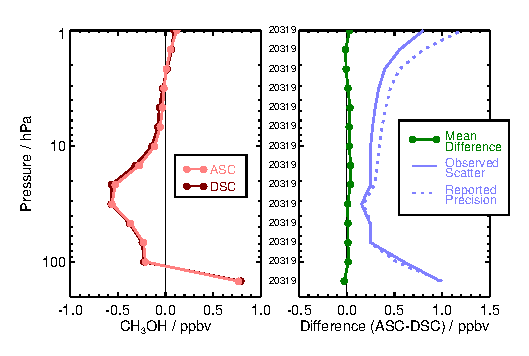
\includegraphics[width=10.0cm]{figures/MLSascdsc_CH3OH_clim}
\caption{(left) Ensemble mean profiles for ascending (light red) and
  descending (dark red) orbit matching pairs of MLS \thisv CH\cs3OH
  profiles averaged over several months of a representative year of
  data (2005).  Symbols indicate MLS retrieval pressure levels.
  (right) Mean differences (ascending$-$descending) in pptv (green
  solid line).  Also shown are the standard deviations about the mean
  differences (light blue solid line) and the root sum square (RSS) of
  the precisions calculated by the retrieval algorithm for the two
  sets of profiles (light blue dashed line). The observed scatter
  about the mean differences and the reported precision values have
  been scaled by 1/$\sqrt{2}$ (to convert from standard deviations of
  differences into standard deviations of individual data points);
  hence the light blue solid line represents the statistical
  repeatability of the MLS measurements, and the light blue dashed
  line represents the expected \mbox{1-$\sigma$} precision for a
  single profile.  The thin black lines mark zero in each panel.  The
  number of crossing pairs of measurements being compared at each
  pressure level is noted in the space between the panels.}
\label{fig:mlsascdscCH3OH}
\end{figure}

The precision of the MLS CH\cs3OH data is estimated empirically by
comparing profiles measured at the intersections of ascending (day)
and descending (night) portions of the orbit. Under ideal conditions
(i.e., a quiescent atmosphere), the standard deviation about the mean
differences between such matched profile pairs provides a measure of
the precision of the individual data points. In practice, however,
real changes in the atmosphere may occur over the 12\,h interval
between the intersecting measurement points, in which case the
observed scatter provides an upper limit on the estimate of precision,
assuming that the a priori has a negligible influence on the retrieval
(a reasonable assumption throughout the retrieval range for
CH\cs3OH). The precision estimates were found to be essentially
invariant with time; results for several months of a representative
year of data are shown in Figure~\ref{fig:mlsascdscCH3OH}.  For the
most part, differences between paired profiles are small, implying the
absence of significant systematic ascending / descending biases. The
observed standard deviation is \texttildelow1\,ppbv at 147\,hPa. The
observationally determined precision agrees well with that reported
for each data point by the Level~2 data processing system.  The
estimates reported here represent the precisions at each pressure
level of a single profile; precision can generally be improved by
averaging, with the precision of an average of $N$ profiles being
1/$\sqrt{N}$ times the precision of an individual profile (although
the actual standard error of the mean can in some cases be even
smaller \citep{TooheyAndVonClarmann13}).

\subsection*{Range}

CH\cs3OH is retrieved (and reported in the Level~2 files) over the
range 147 to 0.001\,hPa.  However, zonal mean mixing ratios are
negative everywhere at retrieval pressures less than 100\,hPa, as well
as at middle and high latitudes at 100\,hPa.  Thus, with rare
exceptions (such as during extreme events), the v4 \meoh\ data are
considered potentially useful for scientific studies only at 147\,hPa
and at lower latitudes at 100\,hPa.

\subsection*{Accuracy}

The impact of various sources of systematic uncertainty has not yet
been quantified for CH\cs3OH as it has for most other MLS products.
This work is planned as part of a dedicated validation exercise for
the \thisv CH\cs3OH data.

\subsection*{Review of comparisons with other datasets}

Detailed comparisons with correlative data sets have not yet been
undertaken.  This work is planned as part of a dedicated validation
exercise for the \thisv CH\cs3OH data.

\subsection*{Data screening}
\begin{description}
\item[Do not use:] Until more comprehensive validation studies have
  been done, the \thisv CH\cs3OH data should only be used in
  consultation with the MLS science team.
\end{description}

\subsection*{Artifacts}
\begin{itemize}
\item A complete assessment of artifacts in the \thisv CH\cs3OH
  measurements has not yet been performed, but it is known that zonal
  mean mixing ratios are negative everywhere at retrieval pressures
  less than 100\,hPa, as well as at middle and high latitudes at
  100\,hPa.
\end{itemize}

\subsection*{Desired improvements for future data version(s)}
\begin{itemize}
\item Specific improvements in the CH\cs3OH retrieval remain to be
  determined.
\end{itemize}

\begin{table*}[bp]
\caption{Summary of Aura MLS \thisv CH\cs3OH Characteristics}\vspace{0.5ex}
\label{tab:CH3OHSummary}
\begin{minipage}{\linewidth}
\renewcommand{\thefootnote}{\thempfootnote}
\centering\begin{tabular}{ccccl}
\toprule
\parbox[m]{18mm}{\bfseries\centering{Pressure\\ / hPa}} &
\parbox[m]{24mm}{\bfseries\centering{Resolution\\ V $\times$ H%
\footnote{Vertical and Horizontal resolution in along-track direction.} \\ / km}} &
\parbox[m]{18mm}{\bfseries\centering{Precision%
    \footnote{Precision on individual profiles.} \\/ ppbv}} &
\parbox[m]{20mm}{\bfseries\centering{Accuracy\\ / ppbv}} &
\parbox[m]{40mm}{\bfseries\centering{Known Artifacts\\ or Other Comments}} \\
%
\midrule
%
68\,--\,0.001  & ---                             & ---      & ---  & Unsuitable for scientific use\\
%
100            & 5         $\times$ 350          & $\pm$1   & TBD  &  \\
%
147            & 4         $\times$ 150          & $\pm$1   & TBD  & \\
%
1000\,--\,215  & ---                             & ---      & ---  & Not retrieved\\
%
\bottomrule
\end{tabular}
\end{minipage}
\end{table*}

%%% Local Variables: 
%%% mode: latex
%%% TeX-master: "v4-x-report"
%%% End: 
